\documentclass[11pt]{article}
\usepackage{geometry}                % See geometry.pdf to learn the layout options. There are lots.
\geometry{letterpaper}                   % ... or a4paper or a5paper or ... 
%\geometry{landscape}                % Activate for for rotated page geometry
\usepackage[parfill]{parskip}    % Activate to begin paragraphs with an empty line rather than an indent
\usepackage{graphicx}
\usepackage{amssymb}
\usepackage{epstopdf}
\DeclareGraphicsRule{.tif}{png}{.png}{`convert #1 `dirname #1`/`basename #1 .tif`.png}

\title{August 27th, 2015 Pre-Class Questions}
\author{Elliot Cartee}
%\date{}                                           % Activate to display a given date or no date

\begin{document}
\maketitle
\subsection*{Question 1}

This plot can be found in Figure $\ref{speedup}$.

\begin{figure}[h]
	\centering
	\caption{\label{speedup}Idealized speedup versus number of cores}
	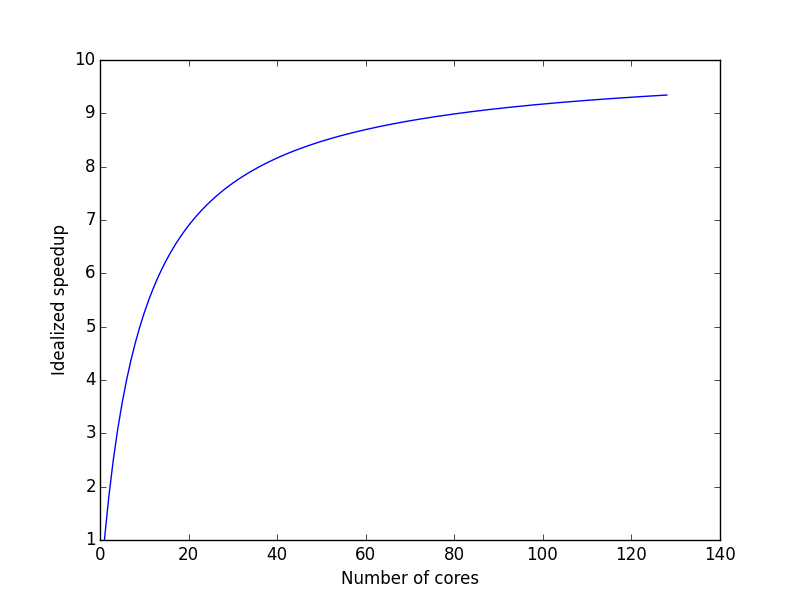
\includegraphics[width=0.8\textwidth]{figure_1.png}
\end{figure}

A script to make the plot using $\begin{tt}matplotlib\end{tt}$ is in $\begin{tt}parallel\_plot.py\end{tt}$ in this directory. It follows here:

\newpage
\begin{verbatim}
import matplotlib.pyplot as plt

max_cores = 128
serial_fraction = 0.1

cores = range(1,max_cores+1)
speedup = range(0,max_cores) #temporary
for i in cores:
	speedup[i-1] = 1.0/(serial_fraction + (1.0-serial_fraction)/i)

plt.plot(cores,speedup)
plt.xlabel('Number of cores')
plt.ylabel('Idealized speedup')
plt.show() 
\end{verbatim}




\subsection*{Question 2}

We note that the serial time required to compute $k$ tasks is $k*\alpha + k*\tau$. The parallelizable part is $k*\tau$. As the number of processors increases, the wall clock time required to complete the parallelizable part goes to 0, and thus the throughput is bounded by $k*\tau/k = \tau$
	
	
\subsection*{Question 3}

It is best not to tune when the human time required to tune is more valuable than the computer time that is saved by tuning.
This can be the case because implementing and maintaining better performance can become very difficult,
or because a particular part of the code does not consume much of the total time

\subsection*{Question 4}

Each of the Xeon Phi 5110P boards has a frequency of 1.053 GHz with 60 cores

Source: 
\begin{verbatim}
http://ark.intel.com/products/71992/Intel-Xeon-Phi-Coprocessor-5110P-8GB-1_053-GHz-60-core
\end{verbatim}
	
Each core can compute 16 double precision floating point operations per cycle

Source: 
\begin{verbatim}
https://software.intel.com/en-us/articles/intel-xeon-phi-core-micro-architecture
\end{verbatim}
	
Each of the 8 nodes has a Intel Xeon E5-2620 v3 processor, which has 12 cores at a base frequency of 2.4 GHz

Source: 
\begin{verbatim}
http://ark.intel.com/products/83352/Intel-Xeon-Processor-E5-2620-v3-15M-Cache-2_40-GHz
\end{verbatim}

The above source also says it uses the AVX 2.0 instruction set. According to the source below, this can compute 16 double precision floating point operations per clock.

Source: 
\begin{verbatim} 
http://www.intel.com/content/dam/www/public/us/en/documents/white-papers/
performance-xeon-e5-v3-advanced-vector-extensions-paper.pdf 
\end{verbatim}

(Note that I had to split the URL into two lines because it is too long for the page)



This means that the theoretical peak flop rate from the accelerators is:
$$
\mbox{(\# of cores)*(cycles per second)*(flops per cycle) } 
$$
$$
= (15*60)*(1.053 \mbox{ GHz})*(16) = 15163.2 \mbox{GFlop/sec} = 15.2 \mbox{TFlop/sec}
$$

And the theoretical peak flop rate from the nodes is:
$$
\mbox{(\# of cores)*(cycles per second)*(flops per cycle) } 
$$
$$
= (8*12)*(2.4 \mbox{ GHz})*(16) = 3686.4 \mbox{GFlop/sec} = 3.7 \mbox{TFlop/sec}
$$

Together this comes out to a theoretical peak flop rate of:
$$15.2 \mbox{TFlop/sec} + 3.7 \mbox{TFlop/sec} = 18.9 \mbox{TFlop/sec} $$

\subsection*{Question 5}

My machine is a mid-2012 13-inch Macbook Air. It has a 1.8 GHz Intel Core i5 processor with two cores
Source: 
\begin{verbatim}
http://ark.intel.com/products/64903/Intel-Core-i5-3427U-Processor-3M-Cache-up-to-2_80-GHz
\end{verbatim}

Since this CPU uses the AVX instruction set, it can execute 8 double precision flops per cycle,
So the theoretical peak flop rate is:
$$
\mbox{(\# of cores)*(cycles per second)*(flops per cycle) }
$$
$$
= (2)*(1.8 \mbox{ GHz})*(16) = 57.6 \mbox{GFlop/sec}
$$





\end{document}  















